
\section{In-silico Results}
We evaluated SeedProteo on two primary tasks: unconditional protein monomer generation and protein binder design. Unconditional generation refers to designing monomeric proteins starting from Gaussian noise, which serves to assess the model's fundamental generative capability. Binder design, on the other hand, involves generating potential high-affinity binders based on the full atomic information of a given target protein, with the goal of enabling real-world applications.

Although numerous diffusion-based co-design methods are capable of jointly generating sequences and structures (in either backbone or all-atom form), existing results consistently indicate that the sequence consistency of their outputs is generally lower than that achieved by redesigning structures using ProteinMPNN \cite{dauparasRobustDeepLearning2022}. Therefore, in the subsequent evaluations, for the structures generated by diffusion-based methods, we employed ProteinMPNN for sequence redesign to ensure fair and comparable assessments. Regarding the details of the evaluation procedure and the definitions of the metrics, please refer to Appendix \ref{app:eval_settings}.

\begin{figure}[t]
    \centering
    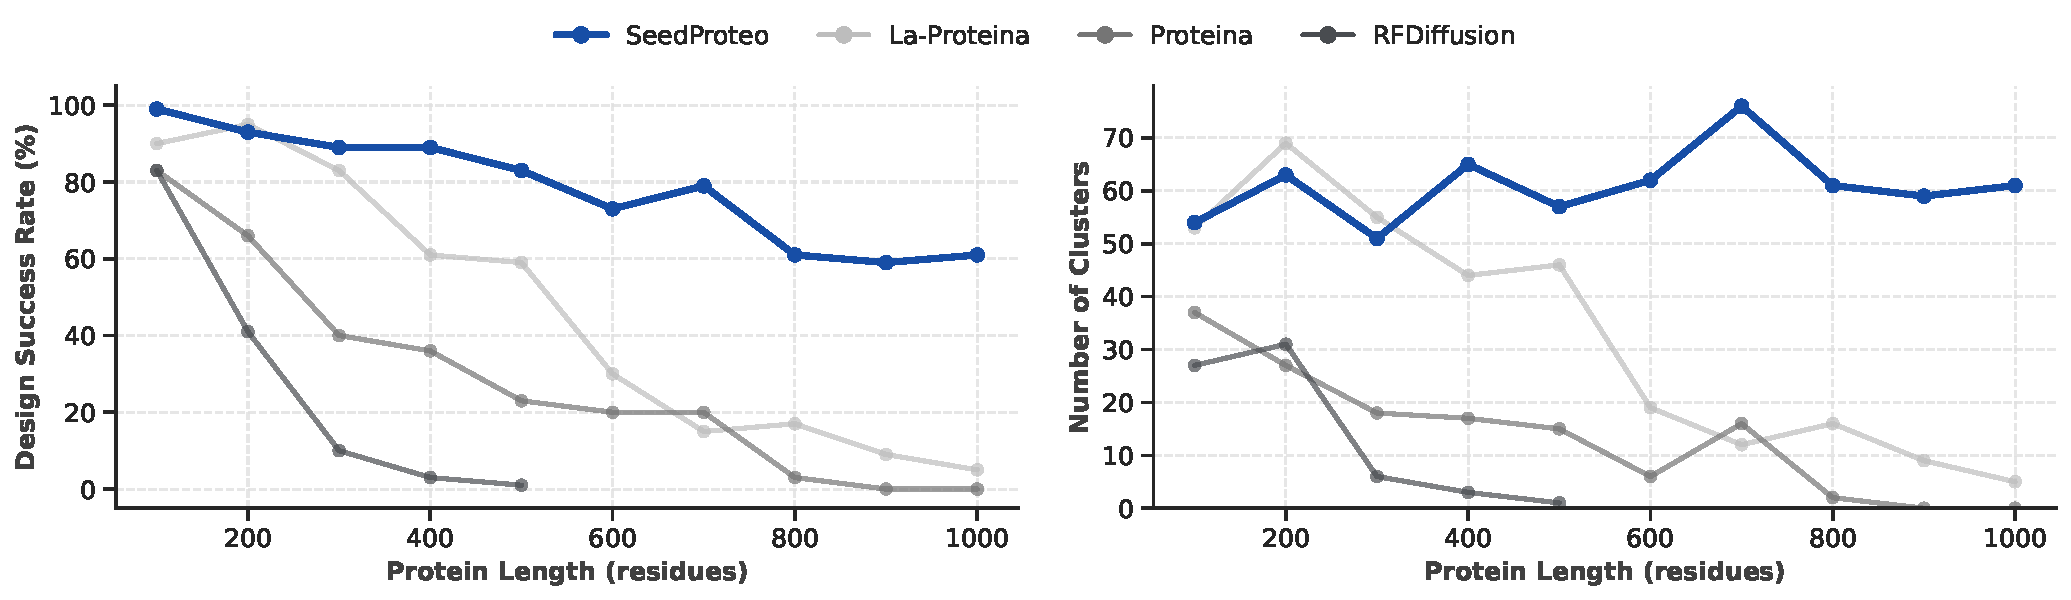
\includegraphics[width=0.98\linewidth]{figures/uncond_perf.pdf}
    \caption{Unconditional monomer benchmark. Stricter thresholds are applied to define designability (in Appendix \ref{app:eval_settings}).}
    \label{fig:uncond_perf}
\end{figure}

\subsection{Unconditional Generation Benchmark}
\subsubsection{Scalability and Structural Diversity}
We first evaluate SeedProteo against state-of-the-art diffusion-based baselines, La-Proteina \cite{geffnerLaProteinaAtomisticProtein2025}, Proteina \cite{geffnerProteinaScalingFlowbased2024}, and RFDiffusion \cite{watsonNovoDesignProtein2023}, on the task of unconditional monomer generation. We focus on two critical dimensions: \textit{scalability} to long sequences and \textit{structural diversity}. As illustrated in Figure \ref{fig:uncond_perf} (Left), SeedProteo consistently achieves superior design success rates across the entire length spectrum (100--1000 residues). While competing methods exhibit a sharp performance degradation as sequence length increases, dropping to near-zero success rates beyond 600 residues, SeedProteo maintains robust performance, achieving a success rate of $>60\%$ even at length 1000. This suggests that our method effectively models the long-range dependencies and global constraints inherent in large protein assemblies, a capability that current baselines lack. In addition to quality, SeedProteo excels in generative diversity. Figure \ref{fig:uncond_perf} (Right) plots the number of unique structural clusters found within the successful samples. Notably, as protein length increases, baselines suffer from severe mode collapse (e.g., RFDiffusion and Proteina generate few to no unique clusters at long lengths). In contrast, SeedProteo sustains a high volume of unique clusters, indicating that it captures a richer and more generalizable distribution of the protein structure space.

\begin{table}[p]
    \centering
    \caption{\textbf{Unconditional Design Benchmark Performance across Structural Topologies.} 
    We compare \textbf{SeedProteo} against baselines on three different fold types: $\alpha$-helix bundles (HHH), Hybrid (HEL), and $\beta$-sheets (EEE). 
    Metrics reported in order: Design Success Rate (\textbf{Succ.}, $\uparrow$), Unique Success Clusters (\textbf{Uniq.}, $\uparrow$), and Novelty (\textbf{Nov.}, $\downarrow$). 
    The best performance is highlighted in \textbf{bold}. Dash (--) indicates model failure or insufficient successful samples.}
    \label{tab:full_comparison}
    
    \resizebox{\textwidth}{!}{%
    \begin{tabular}{l | ccc | ccc | ccc | ccc}
        \toprule
        \multicolumn{13}{c}{\large \textbf{Panel A: Primarily $\alpha$-Helix (HHH) Structures}} \\
        \midrule
        \multirow{2}{*}{\textbf{Length}} & \multicolumn{3}{c|}{\textbf{SeedProteo (Ours)}} & \multicolumn{3}{c|}{\textbf{La-Proteina}} & \multicolumn{3}{c|}{\textbf{Proteina}} & \multicolumn{3}{c}{\textbf{RFDiffusion}} \\
        \cmidrule(lr){2-4} \cmidrule(lr){5-7} \cmidrule(lr){8-10} \cmidrule(lr){11-13}
         & Succ. $\uparrow$ & Uniq. $\uparrow$ & Nov. $\downarrow$ & Succ. $\uparrow$ & Uniq. $\uparrow$ & Nov. $\downarrow$ & Succ. $\uparrow$ & Uniq. $\uparrow$ & Nov. $\downarrow$ & Succ. $\uparrow$ & Uniq. $\uparrow$ & Nov. $\downarrow$ \\
        \midrule
        100 & \textbf{100\%} & 17 & 0.89 & 93\% & \textbf{27} & 0.86 & 88\% & 22 & \textbf{0.83} & 87\% & 19 & 0.89 \\
        200 & \textbf{96\%} & 24 & 0.85 & \textbf{96\%} & \textbf{60} & \textbf{0.80} & 73\% & 21 & 0.83 & 73\% & 8 & 0.85 \\
        300 & \textbf{95\%} & 24 & 0.83 & 85\% & \textbf{47} & \textbf{0.80} & 51\% & 13 & 0.88 & -- & -- & -- \\
        400 & \textbf{98\%} & 32 & 0.79 & 61\% & \textbf{40} & \textbf{0.76} & 39\% & 14 & 0.88 & -- & -- & -- \\
        500 & \textbf{90\%} & 36 & 0.81 & 67\% & \textbf{43} & \textbf{0.74} & 33\% & 12 & 0.85 & -- & -- & -- \\
        600 & \textbf{86\%} & \textbf{38} & \textbf{0.79} & 43\% & 9 & 0.88 & 27\% & 6 & 0.89 & -- & -- & -- \\
        700 & \textbf{86\%} & \textbf{49} & \textbf{0.82} & 38\% & 6 & 0.83 & 24\% & 15 & 0.89 & -- & -- & -- \\
        800 & \textbf{65\%} & \textbf{39} & \textbf{0.79} & 41\% & 10 & 0.86 & 4\% & 2 & 0.96 & -- & -- & -- \\
        900 & \textbf{66\%} & \textbf{45} & \textbf{0.75} & 41\% & 7 & 0.88 & -- & -- & -- & -- & -- & -- \\
        1000 & \textbf{63\%} & \textbf{41} & \textbf{0.77} & 31\% & 5 & 0.88 & -- & -- & -- & -- & -- & -- \\
        
        \midrule
        \multicolumn{13}{c}{\large \textbf{Panel B: Hybrid Helix-E-Loop (HEL) Structures}} \\
        \midrule
        \multirow{2}{*}{\textbf{Length}} & \multicolumn{3}{c|}{\textbf{SeedProteo (Ours)}} & \multicolumn{3}{c|}{\textbf{La-Proteina}} & \multicolumn{3}{c|}{\textbf{Proteina}} & \multicolumn{3}{c}{\textbf{RFDiffusion}} \\
        \cmidrule(lr){2-4} \cmidrule(lr){5-7} \cmidrule(lr){8-10} \cmidrule(lr){11-13}
         & Succ. $\uparrow$ & Uniq. $\uparrow$ & Nov. $\downarrow$ & Succ. $\uparrow$ & Uniq. $\uparrow$ & Nov. $\downarrow$ & Succ. $\uparrow$ & Uniq. $\uparrow$ & Nov. $\downarrow$ & Succ. $\uparrow$ & Uniq. $\uparrow$ & Nov. $\downarrow$ \\
        \midrule
        100 & \textbf{97\%} & 26 & \textbf{0.82} & 87\% & \textbf{27} & 0.86 & 87\% & 13 & \textbf{0.82} & 71\% & 12 & 0.85 \\
        200 & \textbf{92\%} & \textbf{32} & \textbf{0.79} & 90\% & 7 & 0.81 & 55\% & 6 & 0.82 & 38\% & 22 & 0.80 \\
        300 & \textbf{81\%} & \textbf{21} & \textbf{0.77} & 72\% & 8 & 0.83 & 15\% & 4 & 0.85 & 11\% & 6 & 0.78 \\
        400 & \textbf{79\%} & \textbf{26} & \textbf{0.77} & 62\% & 3 & 0.79 & 12\% & 2 & 0.91 & 3\% & 3 & 0.80 \\
        500 & \textbf{69\%} & \textbf{20} & \textbf{0.75} & 60\% & 3 & 0.83 & 5\% & 2 & 0.87 & 1\% & 1 & 0.76 \\
        600 & \textbf{57\%} & \textbf{23} & \textbf{0.77} & 26\% & 12 & 0.85 & -- & -- & -- & -- & -- & -- \\
        700 & \textbf{72\%} & \textbf{28} & \textbf{0.77} & 9\% & 6 & 0.88 & 9\% & 1 & 0.93 & -- & -- & -- \\
        800 & \textbf{56\%} & \textbf{22} & \textbf{0.79} & 11\% & 6 & 0.86 & -- & -- & -- & -- & -- & -- \\
        900 & \textbf{44\%} & \textbf{14} & \textbf{0.78} & 3\% & 2 & 0.89 & -- & -- & -- & -- & -- & -- \\
        1000 & \textbf{57\%} & \textbf{20} & \textbf{0.74} & -- & -- & -- & -- & -- & -- & -- & -- & -- \\
        
        \midrule
        \multicolumn{13}{c}{\large \textbf{Panel C: Primarily $\beta$-Sheet (EEE) Structures}} \\
        \midrule
        \multirow{2}{*}{\textbf{Length}} & \multicolumn{3}{c|}{\textbf{SeedProteo (Ours)}} & \multicolumn{3}{c|}{\textbf{La-Proteina}} & \multicolumn{3}{c|}{\textbf{Proteina}} & \multicolumn{3}{c}{\textbf{RFDiffusion}} \\
        \cmidrule(lr){2-4} \cmidrule(lr){5-7} \cmidrule(lr){8-10} \cmidrule(lr){11-13}
         & Succ. $\uparrow$ & Uniq. $\uparrow$ & Nov. $\downarrow$ & Succ. $\uparrow$ & Uniq. $\uparrow$ & Nov. $\downarrow$ & Succ. $\uparrow$ & Uniq. $\uparrow$ & Nov. $\downarrow$ & Succ. $\uparrow$ & Uniq. $\uparrow$ & Nov. $\downarrow$ \\
        \midrule
        100 & \textbf{100\%} & \textbf{12} & \textbf{0.80} & \textbf{100\%} & 1 & 0.88 & 50\% & 3 & 0.84 & -- & -- & -- \\
        200 & 86\% & \textbf{6} & \textbf{0.80} & \textbf{100\%} & 2 & 0.84 & -- & -- & -- & 20\% & 1 & 0.75 \\
        300 & \textbf{80\%} & \textbf{4} & \textbf{0.80} & -- & -- & -- & 25\% & 1 & 0.85 & -- & -- & -- \\
        400 & \textbf{73\%} & \textbf{7} & \textbf{0.80} & 50\% & 1 & 0.85 & 57\% & 2 & 0.85 & -- & -- & -- \\
        500 & \textbf{50\%} & \textbf{1} & \textbf{0.68} & -- & -- & -- & 50\% & 1 & 0.74 & -- & -- & -- \\
        600 & -- & -- & -- & \textbf{25\%} & \textbf{4} & \textbf{0.86} & -- & -- & -- & -- & -- & -- \\
        700 & -- & -- & -- & \textbf{8\%} & \textbf{1} & \textbf{0.86} & -- & -- & -- & -- & -- & -- \\
        \bottomrule
    \end{tabular}%
    }
    \vspace{0.5em}
    \\
    \footnotesize{\textit{Note: Only lengths up to 700 are shown for EEE as all methods failed to generate valid long $\beta$-sheet structures.}}
\end{table}


\begin{table}[t]
\centering
\setlength{\tabcolsep}{4.5pt}
\renewcommand{\arraystretch}{1.0}

\caption{\textbf{Structural Novelty ($\downarrow$) in Binder Design Benchmark.} Transposed comparison of average novelty scores. We compare \textbf{SeedProteo} variants against baselines across ten targets. \textbf{Lower is Better.} Best performance per target is highlighted in \textbf{bold}, and the second best is \underline{underlined}.}
\label{tab:novelty}

\begin{tabular}{l cccccccccc}
\toprule
\textbf{Method} & \textbf{TrkA} & \textbf{PD-L1} & \textbf{Insulin} & \textbf{BHRF1} & \textbf{IL-7RA} & \textbf{SC2RBD} & \textbf{VEGF-A} & \textbf{H1} & \textbf{IL-17A} & \textbf{TNFA} \\
\midrule
\multicolumn{11}{l}{\textit{\textbf{Ours}}} \\
SeedProteo-D & \underline{0.829} & \textbf{0.832} & \textbf{0.837} & \textbf{0.822} & \textbf{0.840} & \textbf{0.819} & \textbf{0.836} & \textbf{0.823} & \underline{0.806} & \textbf{0.870} \\
SeedProteo-R & 0.905 & 0.913 & 0.911 & 0.872 & 0.917 & \underline{0.858} & 0.901 & 0.890 & 0.855 & - \\
\midrule
\multicolumn{11}{l}{\textit{\textbf{Baselines}}} \\
BindCraft    & 0.849 & 0.856 & \underline{0.864} & 0.847 & \underline{0.861} & 0.863 & \underline{0.850} & \underline{0.830} & 0.818 & -- \\
PXDesign     & 0.914 & 0.929 & 0.928 & 0.924 & 0.928 & 0.917 & 0.913 & 0.888 & 0.906 & -- \\
BoltzGen     & 0.908 & 0.924 & 0.929 & 0.928 & 0.885 & 0.915 & 0.902 & 0.885 & 0.863 & -- \\
RFDiffusion  & 0.932 & 0.934 & 0.927 & 0.946 & 0.916 & 0.912 & 0.940 & --    & 0.938 & -- \\
RFDiffusion3 & \textbf{0.808} & \underline{0.834} & 0.876 & \underline{0.845} & \textbf{0.840} & -- & -- & 0.930 & \textbf{0.800} & -- \\
\bottomrule
\end{tabular}
\end{table}

\subsubsection{Fine-grained Evaluation across Structural Topologies}
Previous generative models often exhibit a strong preference for simple $\alpha$-helical architectures \cite{watsonNovoDesignProtein2023, quPallatomUnlockingNew2025}, frequently failing to generalize to complex topologies such as all-$\beta$ sheets. Our empirical observations confirm that designability is highly topology-dependent: primarily $\beta$-sheet structures consistently yield lower success rates compared to helical bundles across all models. To dissect this phenomenon, we present a fine-grained evaluation in Table \ref{tab:full_comparison}, breaking down performance by three distinct topologies: primarily $\alpha$-helix (HHH), primarily $\beta$-sheet (EEE) and hybrid Helix-Sheet-Loop (HEL). The results reveal a distinct advantage for SeedProteo in handling complex folds:

\begin{itemize}
    \item \textbf{Complex Topology Robustness:} In the Hybrid (HEL) category, SeedProteo achieves a 57\% success rate at length 1000, whereas baselines largely fail to produce valid structures beyond length 600.
    
    \item \textbf{$\beta$-Sheet Generation:} In the $\beta$-sheet (EEE) regime, which is notoriously difficult for generative models, SeedProteo is the only method capable of generating diverse, valid and novel structures (Success $>50\%$ and Novelty $<0.8$) at lengths up to 500. Other models suffer from complete generation failure or mode collapse in this category.
    
    \item \textbf{Novelty and Diversity:} Across all topologies, SeedProteo consistently achieves higher structural diversity (Unique Clusters) and favorable novelty scores, indicating that it does not merely retrieve training templates but effectively explores novel regions of the protein manifold.
\end{itemize}

\subsection{Binder Design Benchmark}
We benchmark SeedProteo against five leading open-source binder design methods: RFDiffusion \cite{watsonNovoDesignProtein2023}, RFDiffusion3 \cite{butcher2025novo}, BoltzGen \cite{starkUniversalBinderDesign}, PXDesign \cite{ren2025pxdesign}, and BindCraft \cite{pacesaOneshotDesignFunctional2025}. Following the protocol established in AlphaProteo \cite{zambaldi2024novo}, we generate approximately 1,000 candidates for each of the 10 benchmark targets, uniformly covering the target-specific binder length ranges. For structure-generating diffusion models (SeedProteo, RFDiffusion variants, PXDesign, and BoltzGen), binder sequences are redesigned using ProteinMPNN. A notable exception is BindCraft, a hallucination-based approach \cite{anishchenkoNovoProteinDesign2021}, which optimizes sequences directly via gradient descent on folding metrics (e.g., ipTM). All designs are subsequently evaluated \textit{in silico} using SeedFold \cite{seedfold}. We adopt the success criteria defined in AlphaProteo: minimum inter-chain Predicted Aligned Error (PAE) $\le 1.5$, binder pTM $\ge0.8$, and complex RMSD $<2.5$\AA.

In SeedProteo, we introduce two distinct Secondary Structure (SS) sampling modes to balance the trade-off between designability and structural diversity: 
\begin{itemize} 
    \item \textbf{SeedProteo-R:} This is a SS robust mode. Prioritizes fewer but longer continuous secondary structure segments. This mode imposes stronger structural stability constraints, typically yielding a higher design success number. 
    
    \item \textbf{SeedProteo-D:} This is a SS diverse mode. Allows for a higher frequency of shorter secondary structure segments. This mode encourages more complex topologies, resulting in greater structural diversity at the cost of slightly reduced raw success number. 
\end{itemize}


\paragraph{Performance Analysis.} We evaluated the unconditional generation capabilities of SeedProteo across a diverse set of ten target proteins. As shown in Figure \ref{fig:front}, SeedProteo-R demonstrates a commanding lead in total success counts across the benchmark. Notably, this advantage is most pronounced on challenging targets, specifically SC2RBD, VEGF-A, H1, and TNF$\alpha$.

Beyond design success, structural diversity is a critical metric for downstream applicability. Figure \ref{fig:front} highlights that \texttt{SeedProteo-D} excels in generating structurally distinct binders, achieving the highest number of unique success clusters in 8 out of the 10 targets. Complementing this structural diversity, Table \ref{tab:novelty} demonstrates that SeedProteo-D also achieves the best novelty scores for successfully designed binders in 8 out of the 10 targets. Notably, it consistently outperforms all baselines, except RFDiffusion3, across every target; for example, while baselines like PXDesign often yield scores above 0.9, SeedProteo-D maintains superior novelty with scores in the 0.8 range. This indicates that SeedProteo does not merely converge on a single solution but effectively explores the structural landscape to provide a diverse portfolio of high-quality and novel candidates. Figure \ref{fig:case} presents case studies on challenging targets.


\begin{figure}[t]
    \centering
    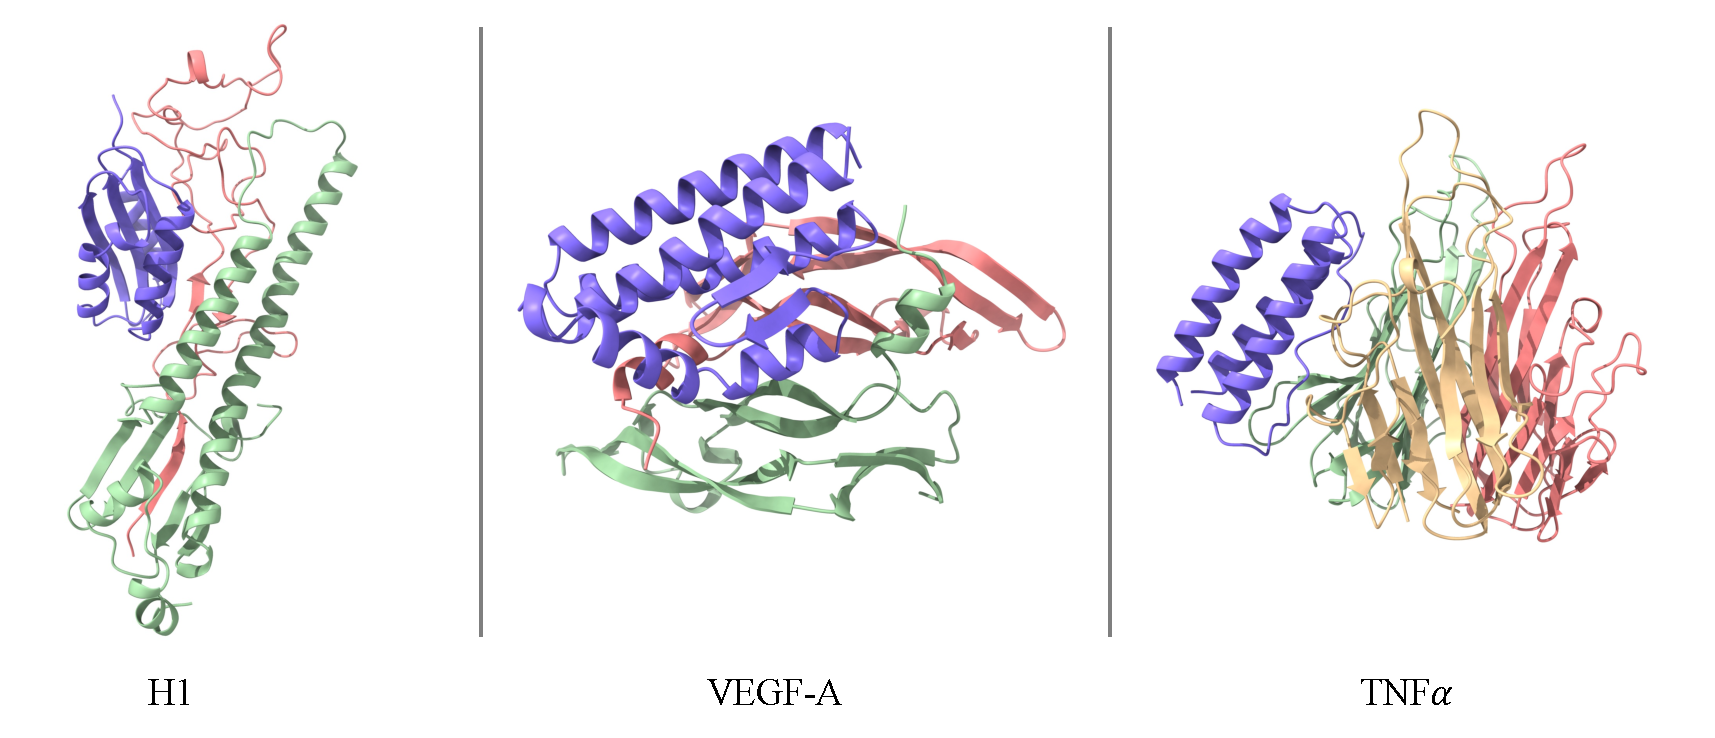
\includegraphics[width=0.90\linewidth]{figures/case.pdf}
    \caption{Binders generated by SeedProteo for the challenging multi-chain targets H1 (dimer), VEGF-A (dimer), and TNF-$\alpha$ (trimer). All displayed binders, colored in purple, meet the in silico success criteria.}
    \label{fig:case}
\end{figure}

\begin{table}[t]
\centering
\caption{\textbf{Benchmarking Co-design Capabilities of Diffusion-based Models for Binder Design.}}
\label{tab:codesign_benchmark}
\resizebox{\textwidth}{!}{%
\begin{tabular}{lcccccccccc}
\toprule
\textbf{Method} & \textbf{BHRF1} & \textbf{SC2RBD} & \textbf{IL-7RA} & \textbf{PD-L1} & \textbf{TrkA} & \textbf{Insulin} & \textbf{H1} & \textbf{VEGF-A} & \textbf{IL-17A} & \textbf{TNF$\alpha$} \\
\midrule
\multicolumn{11}{l}{\textit{Baselines}} \\
BoltzGen & \textbf{627} & 0 & 10 & 17 & 21 & 99 & 1 & 1 & 5 & 0 \\
RFDiffusion3 & 9 & 0 & 0 & 1 & 0 & 0 & 0 & 0 & 0 & 0 \\
\midrule
\multicolumn{11}{l}{\textit{SeedProteo (Ours)}} \\
SeedProteo-R & 296 & \textbf{92} & \textbf{100} & \textbf{380} & \textbf{232} & \textbf{303} & 16 & \textbf{127} & \textbf{47} & 1 \\
SeedProteo-D & 139 & 80 & 52 & 265 & 143 & 181 & \textbf{25} & 45 & 17 & \textbf{3} \\
SeedProteo-M & 133 & 77 & 25 & 154 & 143 & 189 & 12 & 47 & 13 & 1 \\
\bottomrule
\end{tabular}%
}
\end{table}


\begin{table}[t]
\centering
\caption{\textbf{Ablation Study on Sequence Decoding Strategies.}}
\label{tab:ablation_mrf}
\begin{tabular}{l l cccc}
\toprule
\textbf{Length} & \textbf{Decoding Method} & \textbf{scRMSD} $\downarrow$ & \textbf{scTM} $\uparrow$ & \textbf{pLDDT} $\uparrow$ & \textbf{Succ. Rate} $\uparrow$  \\
\midrule
\multirow{2}{*}{100} 
& Baseline (\texttt{atom14}) & \textbf{1.11} & \textbf{0.94} & 88.56 & \textbf{0.90} \\
& SeedProteo (MRF)  & 1.63 & 0.93 & \textbf{88.65} & 0.84 \\
\midrule
\multirow{2}{*}{200} 
& Baseline (\texttt{atom14}) & 3.87 & 0.86 & 78.06 & 0.68 \\
& SeedProteo (MRF)  & \textbf{2.08} & \textbf{0.92} & \textbf{84.36} & \textbf{0.80} \\
\midrule
\multirow{2}{*}{300} 
& Baseline (\texttt{atom14}) & 4.71 & 0.83 & 73.40 & 0.52 \\
& SeedProteo (MRF)  & \textbf{2.30} & \textbf{0.91} & \textbf{80.33} & \textbf{0.76} \\
\bottomrule
\end{tabular}%
\end{table}


\subsection{Discussion on Co-Design Strategies}
We here discuss the significance of co-design and methods for enhancing co-design capabilities. While two-stage pipelines (backbone generation followed by inverse folding) have dominated recent protein design benchmarks, our analysis suggests that simultaneous sequence-structure generation (co-design) offers potential advantages for complex targets.

\paragraph{Beyond the Inverse Folding Bottleneck}
Empirical results (Figure \ref{fig:front} and Table \ref{tab:codesign_benchmark}) indicate that, on average, sequences derived from ProteinMPNN achieve higher success rates than those generated via pure co-design. This is expected, as ProteinMPNN is highly optimized for fixed-backbone recovery. However, we argue that reliance on inverse folding alone is not the ultimate solution for de novo binder design.

A striking exception is observed with the TNF$\alpha$ target. Here, ProteinMPNN-based methods almost universally fail (0 or 1 success) shown in Figure ~\ref{fig:front}, whereas our co-design approach yields valid binders. We reason that inverse folding models tend to fall into "safe" local minima, generating sequences with repetitive motifs (e.g., excessive electrostatic patterns like poly-EK or hydrophobic poly-A stretches) that optimize theoretical likelihood but fail restricted biophysical binding constraints for difficult targets. In contrast, co-design learns to exploit more complex sequence patterns that are still compatible with the structural constraints of the backbone, allowing the model to navigate out of the structural bottlenecks that trap fixed-backbone sequence designers.

\paragraph{Decoding Mechanisms}
We further compare the co-design mechanisms of SeedProteo with diffusion-based baselines, including RFDiffusion3 and BoltzGen, while excluding PXDesign and RFDiffusion as they are limited to backbone design rather than all-atom modeling. Both RFDiffusion3 and BoltzGen utilize variants of the \texttt{atom14} schema, relying on removing specific virtual atoms to implicitly decode amino acid types. In contrast, SeedProteo employs \texttt{atom14} strictly as a geometric input representation, while the final sequence identity is inferred via a Markov Random Field (MRF) module. This allows our model to capture higher-order residue dependencies that simple geometric decoding might miss. 


\subsection{Ablation Study}
\paragraph{Impact of Secondary Structure Constraints}
To evaluate the specific contribution of secondary structure (SS) constraints, we compare our approach against a baseline termed \texttt{SeedProteo-M}, which performs binder design using fully masked SS sequences as condition. As shown in Table \ref{tab:codesign_benchmark}, incorporating secondary structure (SS) sequences as conditioning constraints significantly enhances design success. This constraint effectively prunes the search space, guiding the diffusion process toward \textit{de novo}-like fold topologies.

\paragraph{Impact of MRF module}
To validate the effectiveness of our sequence decoding module, we conducted a supplementary ablation study on unconditional generation (Table \ref{tab:ablation_mrf}). We established a baseline that predicts amino acid identities by aggregating features from the \texttt{atom14} representation at each residue position, a strategy adopted by the recent method \cite{quPallatomUnlockingNew2025}.

As shown in Table \ref{tab:ablation_mrf}, while the baseline achieves competitive performance on short sequences (Length 100), its capability degrades significantly as protein size increases. We reason this divergence to the inherent limitations of the decoding receptive fields. The \texttt{atom14} schema relies on recognizing amino acid types via local side-chain geometry (implicit conformational recognition). However, the underlying AF3-based architecture primarily models pairwise inductive biases and may lack the capacity to capture long-range atomic dependencies solely through local atoms aggregation. Consequently, the baseline struggles to maintain global consistency in larger systems. Conversely, the MRF module explicitly leverages global pairwise features during inference. By modeling the sequence distribution conditional on the entire backbone topology, the MRF ensures that the generated sequence is self-consistent with long-range structural constraints, thereby preventing the structural degeneration observed in the baseline at longer lengths.


